\section{Experiments}
\label{sec:experiments}

We randomly split the following data sets into training sets $80\%$ and
testing sets $20\%$. For multi-class data sets we do one-vs-all (OVA)
classifiers. For approximations that has reasonable run time, we will perform
cross-validation to select parameters for prior, which may have profound
impact on the result as suggested by~\cite{Asuncion2009smoothing}. 

\subsection{Data Sets}


We use 5 \href{http://archive.ics.uci.edu/ml/datasets.html}{UCI classification
datasets}:, described as follows:

\begin{tabular}{| c | c |  c |}
\hline
Dataset & \# instances & \# features \\
\hline
Farms Ads dataset & 4,143 & 54,877 \\
\hline
Amazon Commerce reviews dataset & 1,500 & 10,000 \\
\hline
p53 Mutants dataset & 16,772 & 5,409 \\
\hline
Human Activity Recognition using Smartphones dataset & 10,299 & 561\\
\hline
URL Reputation dataset\footnotemark[1] & 2,396,130 (16000) & 3,231,961 (74113) \\
\hline
\end{tabular}

\footnotetext[1]{The dataset is too large so we used only one day of data out of totally 121 days in the dataset. See number in parentheses for specifications.}

\subsection{Results}

We perform Laplace approximation, which has predictive distribution equivalent
to the MAP estimate under the same approximation. Fig.~\ref{fig:laplace} shows
that the classifier perform reasonably well on both data sets. Moreover, since
our data sets are high dimensional, it is paramount to avoid overfitting. The
classification error on test and training sets are close, demonstrating that
our prior is sufficient for these data sets. Currently we are using $\sigma =
0.05$, which is a relatively concentrated prior. As the next step we would
like to employ cross validation to select an optimal prior covariance $\sigma$.

Even though the data set is intrinsically large, fig.~\ref{fig:laplace} shows
that training on a single machine is reasonably fast. Note that training
converges in 172 and 209 iterations for p53 and farm ads data set,
respectively. Thus the run time {\em per} iteration is comparable: about $5$
seconds per iteration.


\begin{figure}[t]
\label{fig:laplace}
\centering
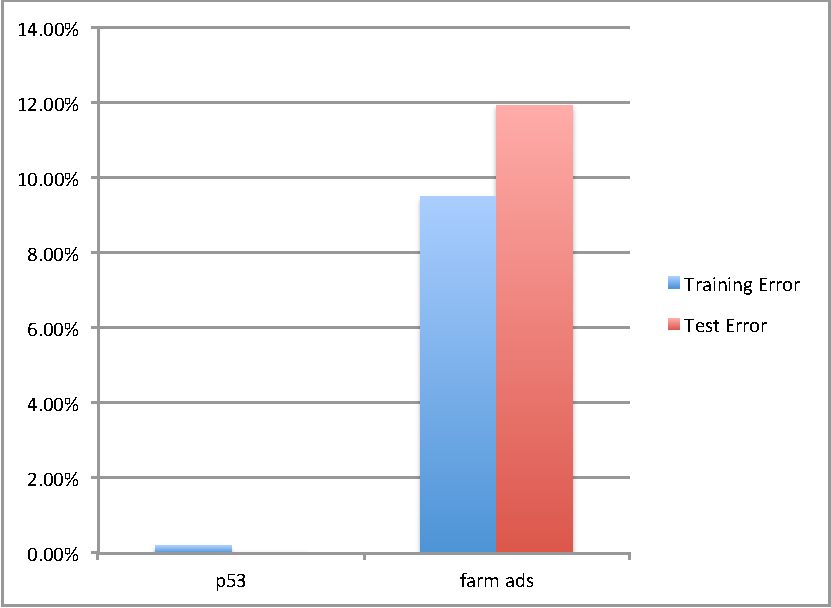
\includegraphics[height=5.0cm]{../../results/classificaiton_errors.pdf}
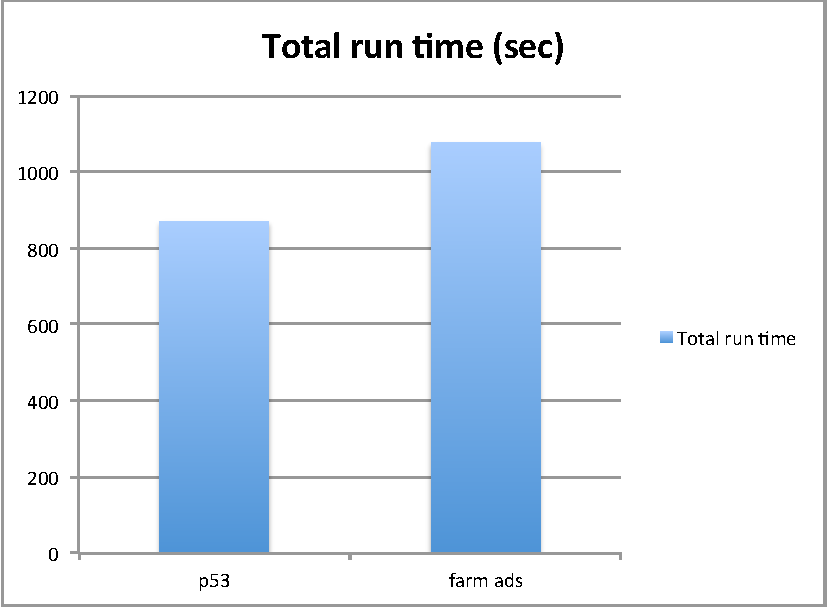
\includegraphics[height=5.0cm]{../../results/runtime.pdf}

\caption{\small On p53 and farm ad data sets; {\bf Left:} Classification errors on
training and testing set using Laplace approximation (or equivalently, the
MAP estimate). {\bf Right:} Training time for each data set. }

\label{graphlab}
\end{figure}

\subsubsection{MCMC based estimation}
Our MCMC sampling strategy that we described in section~\ref{sec:MCMCmethod}
converges. Figure~\ref{fig:MCMCconverge} is a plot of the iterations of the Markov 
chain for estimation on a subset of Farms Ads dataset. This is for MLE
estimation without any priors. We also 

\begin{figure}![htb]
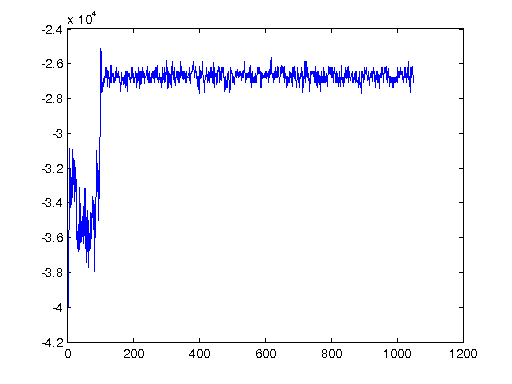
\includegraphics[width=1\textwidth]{samplingConvergence.png}
\caption{Markov chain convergence on Farms ads data. We take a sub-sample of
the dataset: 2000 rows and 100 columns}
\label{fig:MCMCconverge}
\end{figure}
